\documentclass{article}
\usepackage[pdftex]{graphicx}
\usepackage{fixltx2e}
\usepackage{float}
\usepackage{hyperref}
\usepackage[top=1in, bottom=1in, right=1.25in, left=1.25in]{geometry}
\usepackage[usenames, dvipsnames]{color}

\begin{document}

	% Title Page
	\begin{titlepage}

		\title{\textbf{BU ProPane Project Background}}
		\author{BU ProPane Team:\\Griffin Dunn\\Colin Madigan\\Phillip Stahlfeld}
		\date{September 12, 2012}
		\maketitle
		\noindent
		The purpose of this document is to introduce the BU ProPANE project to a third party with no prior knowledge concerning the project. The document begins with a high-level discussion of the problems that this project is aiming to solve. Next, the document provides relevant background information regarding current practices and relevant terminology. The document concludes with a technical research section that contains ideas that will prove useful during the implementation phase of the project. 
		
		\thispagestyle{empty}
	
		
	\end{titlepage}



	\thispagestyle{empty}
	\section*{Problem Statement}
		The goal of this project is to create a system that captures all of the information written on a board during a class in a readily accessible manner. The two driving forces behind solving this problem are: autonomous collection of notes for students with disabilities and providing a means for professors to compare their notes with the actual information presented during a lecture.\\
		\\
		Current practices at Bucknell rely on the aid of a student volunteer to provide photocopies of his or her notes to students who are incapable of taking notes themselves during the class. This is not an optimal solution because: the student volunteer must be in class every day, turnaround time for the notes is too long, and the quality of the student volunteer notes cannot be guaranteed. In addition, several professors use different colored writing to represent different forms of information. If the student volunteer did not copy the notes in color, then any students using the notes would not have access to the same information.\\
		\\
		Typically, professors have a lecture planned out before class starts and have notes prepared to follow their plan. However, when students ask unexpected questions or do not fully grasp the material, it is easy to deviate from this plan. For example, civil engineers at Bucknell University plan out their lectures by dividing a piece of paper into sixths and filling in each block with what they want to present (See Figure \ref{fig:cive-notes}). Problems arise when information not included on these pieces of paper are written on the board (due to student questions etc.). When the professor is preparing to give the lecture the following year, he or she will have to remember what the previous year's students struggled with. Using a board capture system, professors could compare previous lectures with previous lecture notes to generate a more effective lecture plan. 
		
		% Image of Professor Gabauer's lecture notes
		\begin{figure}[h]
      			\centering
      			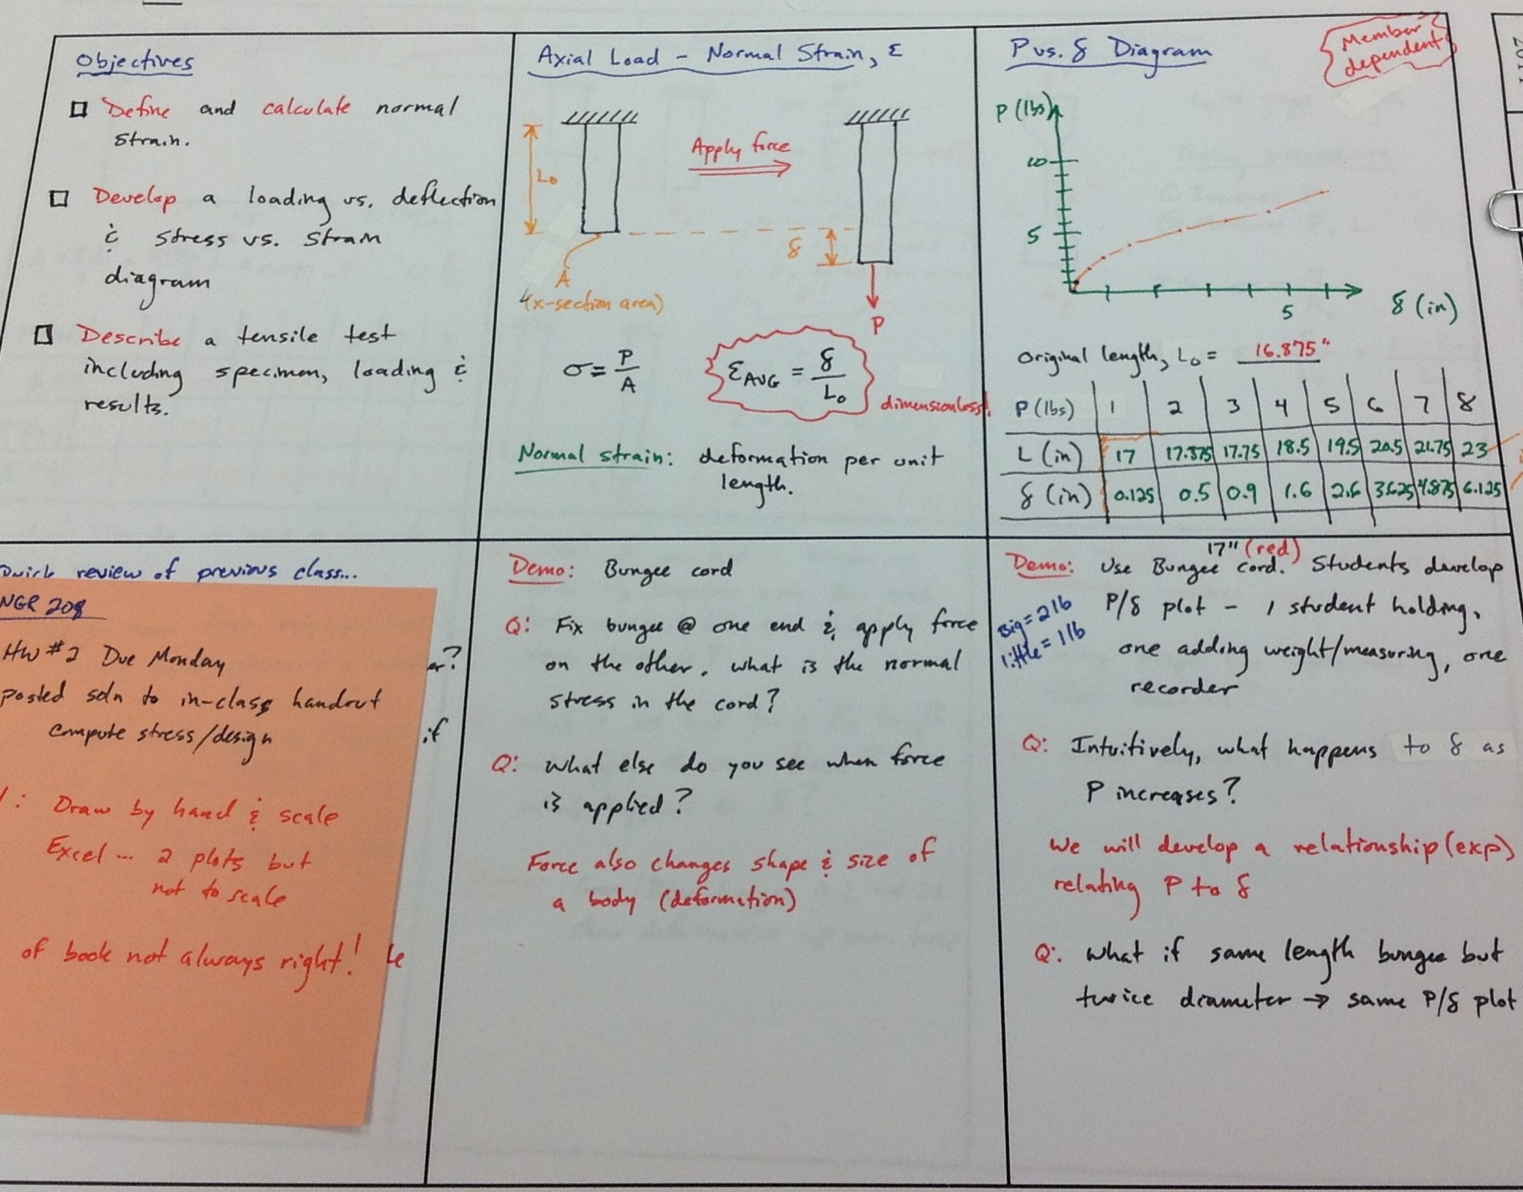
\includegraphics[scale=0.2]{./images/cive-notes.png}
			\caption{Image of civil engineering lecture notes. Orange note is an example of how lecture notes are recorded and altered. Image courtesy of Doug Gabauer 2012.}
			\label{fig:cive-notes}
   		 \end{figure}
		
	\section*{Background Information}
		\subsection*{How are things currently done?}
			Smart phone apps\\
			Professional scribes
			
		\subsection*{Useful Terminology}
			WE WILL GET THIS WITH MORE RESEARCH
	
	\section*{Research}
		\subsection*{Competing Technologies}
			There are three general categories: phone apps, scanners, and electronic whiteboards.\\
			\\
			% Phone apps
			\emph{Phone Apps-}\\
			Phone apps scan an image of a whiteboard and filter out the unnecessary information (See Figure \ref{fig:wbcp-example-ad}). Several examples of phone apps are listed below.
			\begin{itemize}
				\item \href{http://www.beetlebugsoftware.com}{WhiteBoard Capture Pro}
				\item Qipit WHite
				\item Genius Scan
				\item JotNot Scanner Pro
			\end{itemize} 
			
			
			% Scanners 
			\noindent \emph{Scanners-}\\
			Scanners are pieces of hardware that attach to white boards that will tracks movements on the board (some with the usage of an electronic pen). These products will not be fully suited to this project because they require installation and calibration, which violates the idea of portability. Several examples of scanners include:
			\begin{itemize}
				\item MimioCapture
				\item eBeam System 3
				\item Interlink
				\item FreeBeam
			\end{itemize}
			
			
			% Image of WhiteBoard Capture Pro
			\begin{figure}
	      			\centering
	      			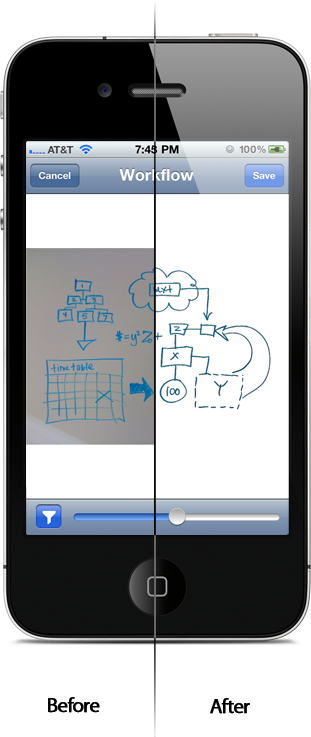
\includegraphics[scale=0.3]{./images/wbcp-example-ad.png}
				\caption{Advertisement demonstrating the image filtering capabilities of the WhiteBoard Capture Pro iPhone app. App eliminates discoloration of board due to glare. Taken from \url{http://www.beetlebugsoftware.com.}}
				\label{fig:wbcp-example-ad}
	   		 \end{figure}
			
		
		\noindent \emph{Electronic Whiteboards-} \\
Smartboards are full sized, touch sensitive whiteboards. You can project images onto them with a projector and then make edits/additions to them with any pointed object. The touch sensitive board senses where you are writing on the board and adds electronic corrections to the image/document. These devices do not compete as directly with our project as the smartphone apps and the scanners because they are not nearly as portable. They are the size of a standard whiteboard and thus cannot be easily moved between classrooms.
            \begin{itemize}
                \item SMART Board
                \item Panasonic's Panaboard
                \item Hitachi's Starboard
                \item The Promethean Board
            \end{itemize}
			
		\subsection*{Research Data}
		
			\subsection*{Smartphone Applications}

			\subsection*{Introduction}
The following paragraphs are descriptions of several smartphone apps that contain features wish to emulate in our own project. They in many ways solve the needs of our current clients. We therefore hope to take some of these phone-app features and modify them to better meet the needs of our own clients. \\
				\subsection*{Whiteboard Capture Pro}
Source: Beetlebug Software's website\\
{\color{red} \url{http://www.beetlebugsoftware.com/}} \\
					
This is an iPhone app that takes a picture of a white board and then analyzes it for key content. The user selects objects to remove from the photograph. This leaves only the writing on the board behind. The App then analyzes the writing and removes the background image of the whiteboard itself. This sometimes leaves fuzz or imperfections in the white background, so there is then a slider available to filter out this extra noise/fuzz that shows up in the end product. The resulting image is a pure white background with handwriting on it.These photos can then be saved, cropped, shared, and organized within-app tools. \\
				\subsection*{WBConference}
Source: Elecom'e website\\
{\color{red} \url{http://app.elecom.co.jp/en/wbcap/ios/manual.html}} \\
					
This is an Android app that competes with our product because it is another whiteboard capturing device. WBConference differs from Whiteboard Capture Pro in that it is able to automatically recognize which sections of the board are whiteboard. This then allows it to apply its ìmagnified keystone correctionî to remove the excess background imagery. In cases that it cannot recognize the board you can zoom in on just the board boundaries manually before capturing the image. The app has contrast adjustment and image rotation as well so you can take images from any orientation without problems.This app has editing features as well so you can add postscripts or speech bubbles to the images. The files can then be saved as PDFs along with any notes you want to add to them.This app has a widget for the home screen for quick image capturing, and you can set up an email address for quick delivery of the images to an external source. \\
				\subsection*{CamScanner -Phone PDF Creator}
Source: Intsig's Website
{\color{red} \url{http://www.intsig.com/en/camscanner.html}} \\
					
This is the most downloaded ëscannerí app on the market. With it you can take photos of any document, whiteboard, etc that you want. You then go through an editing process in which you can select the important portion of the photograph, change the detail level, contrast, light/darkness etc. It will then save your new document in any number of saved folders. You can make notes about each image and these notes will be saved with the image. You can email, print, fax, or transfer via Bluetooth any of the photos. You can also upload your images to google docs, evernote, skydrive, dropbox, or box.net. These documents get saved as PDFs. There are different enhancement modes: No enhance, low and high enhance, gray mode, and B\&W Document modes. These different modes will be better depending on the environment or object that youíre trying to scan. The B\&W mode is particularly helpful when scanning books/papers because it does a better job of removing the background noise. This app allows for batch photo taking and batch photo scanning, so you can take multiple pictures and it will scan them all at the same time. \\
				\subsection*{Whiteboard Capture Pro}
Source: Magnicode's website\\
{\color{red} \url{http://www.magnicode.com/}} \\
					
This app is a dumbed down version of the previous three. It does the job, it scans and enhances images, it just isnít as well known as the others and thus doesnít have the money/time to invest in extra features. This aside, it does work, it is free, and it does save images as PDFs for later use. You can email these photos to yourself and store them in different photos. You can attach notes to your images and you can enhance the quality of the whiteboard picture with their auto-enhance tool. On the upside, it IS a much smaller program than your avg whiteboard capture app. Over all a smaller lighter free alternative. I installed this app on my phone and I had trouble using it because it kept crashing. \\

     \subsection*{Conclusion}
These smart phone apps will be some of the greatest competition to our project because they meet many of our client's needs already. Not only that, they're free applications so our clients wouldnt need to spend money either. The following is a list of features that we should attempt to emulate when designing our own product.

All of these applications contain ways to filter out background noise so that whiteboards appear pure white and text looks crisp and clean. This will be an important aspect of our own product because our image capture device will be subject to a wide variety of lighting situations and will need to be able to adapt to any of them.
Another key feature is the ability of these apps to save and send the images via email, google docs, and other online mediums. This will be an important point in our project as well.
Another good feature was the ability for some of the apps (CamScanner for example) to correct for image angles. If the board is photographed from an angle, the smartphone apps will compensate so that the final scanned image looks like it was taken straight on. \\

        \emph{Desirable features not found in smartphone apps:}
        \begin{itemize} \itemsep -2pt
            \item Photo splicing: These apps do not combine images to add in details covered by professor's body.
            \item Automatic: These apps do not automatically capture images, process them, and then send them away. They instead require user feedback every step of the way.
        \end{itemize}

By adding these features to the functionality currently found in modern apps we hope to create value for our customer.


			\subsection*{Microsoft Whiteboard Capture System}
Source: Microsoft Research Technical Report MSR-TR-2002-89 \\
{\color{red} \url{ftp://ftp.research.microsoft.com/pub/tr/tr-2002-89.pdf}} \\
All images used in this section are from the source document.
		\subsubsection*{Summary}
The Whiteboard Capture System came out of Microsoft Research in 2002.  It was research for a bigger Distributed Meetings project.  It can record all information placed on a whiteboard during a session, as well as the audio in the room, and it provides a platform for users to review key information from the session later from their own computers. 
	
		\subsubsection*{Key Features}
The Whiteboard Capture System (WCS) requires only a camera, microphone, and computer to operate with any existing whiteboard.  It records all information written on the board during a meeting, and all audio in the room during the meeting.  The system then analyzes the data and detects ``key frames'', or pictures of the board which the system determines to contain the most important information.  The key frames are time-stamped so they can be associated with the audio that was recorded at the same point in time.  Users can access the key frames securely via a web-based browsing system.  Audio can be played by clicking on a key frame, and the option exists for the presentation to unfold for the viewer like a movie, where information will appear on their web-based whiteboard as the audio recording talks about it, as shown below in Figure 1.
    
\begin{figure}[H]
\centering
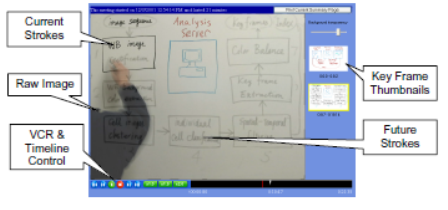
\includegraphics[scale=0.80]{images/research_mswhiteboard_1}
\caption{Browsing system representation of meeting playback}
\end{figure}

		\subsubsection*{Technical information}
The WCS uses a Canon PowerShot G2, a 4 megapixel digital still camera.  The camera provides images with 2272 x 1704 pixel resolution, equivalent to 31.6 dpi for a 6' x 4' whiteboard.  The camera is controlled via USB by a computer, which utilizes the available SDK for the camera to communicate.  It takes a picture roughly every 5 seconds, which is as fast as possible for the PowerShot G2.  Software specifies camera parameters on a per-shot basis.  Pictures are saved as JPEGs and sent to the computer via USB.  The computer is a Pentium III 800 MHz dual CPU PC.  It takes approximately 20 minutes of processing for every hour of session time.  The input image sequence requires 34 MB/hour using motion JPEG compression, while the audio requires 15 MB/hour to store 16-bit 11 KHz mono mp3 audio.  \\

To analyze the captured images, the WCS first divides the frame into a grid of rectangular cells of approximately 1.5'' x 1.5'' inches.  The frame is represented by a 3D matrix of cell images.  Analysis using cells requires much less computational power compared to a per-pixel analysis.  Once the frame is divided into cells, the system uses an algorithm to prepare key frames in a readable fashion.  The algorithm is as follows:

\begin{enumerate} \itemsep -2pt
\item \textbf{Rectify} the whiteboard region of every image in the sequence
\item \textbf{Extract} the whiteboard background color
\item \textbf{Cluster} the cell images throughout the sequence for the same cell. If two images are considered to be the same, they are clustered in the same group.
\item \textbf{Classify} each cell image as a stroke, a foreground object, or the whiteboard
\item \textbf{Filter} teh cell images both spatially and temporally to refine the classification results.
\item \textbf{Extract} the key frame images using the classification results
\item \textbf{Color-balance} the key frame images
\end{enumerate}



	\textbf{1.} To rectify the whiteboard region, they use a one-time calibration step where the corners of the board are selected to manually define the frame.  \\
	\indent \textbf{2.} The whiteboard color is computed by finding cells with the brightest luminance over time and small variance.  During this step, cells which are impeded during the capture process (for example, by a person standing in front of the board) act as outliers.  These are detected and accounted for using a least-median-squares technique.  \\
	\indent \textbf{3.} Cell images are clustered together if they are determined to be identical.  This is determined by a modified Normalized Cross-Correlation algorithm and the use of the Mahalanobis distance calculation.  \\
	\indent \textbf{4.} Cells are classified as whiteboard, stroke, or foreground cells.  Heuristically, whiteboard cells are uniform in color, either white or grey.  Stroke cells are mostly white or grey with one or two primary colors mixed in.  Foreground cells do not fit either of these descriptions.  Essentially, it determines if a cell image is the same as a whiteboard cell image, very similar to a whiteboard cell image (stroke), or completely different (foreground object). \\
	\indent \textbf{5.} Filtering is used to better define cells.  The system's spatial filter changes totally isolated foreground cells to stroke cells, since typically foreground cells are clustered (i.e. a person).  Stroke cells touching foreground cells are also changed to foreground cells, unless said cells are also filtered temporally.  The temporal filter looks at all cell images for a certain cell over time.  If two cell images match, all cell images in between are deemed to be the same image as well.  This filters out foreground objects.  \\
	\indent \textbf{6.} Key frames are considered a summary of the entire presentation.  The WCS defines key frames as frames that capture all information on the board just before an erase.  They should only contain whiteboard and stroke cells, the whiteboard color should be uniform and the pen colors should be distinct.  Image reconstruction is used to ensure the quality of the key frames.  If the cell image is a whiteboard or stroke, its own image is used.  If it's a foreground object within the span of a stroke, it is replaced with the stroke image from the neighboring frame.  Otherwise, it is replaced by a whiteboard cell image.  Key frames are only present before large erases, so they are only identified if at least 20\% of the total stroke count is erased.  The WCS divides the presentation into chapters, with each chapter being concluded by a key frame. 
\begin{figure}[H]
\centering
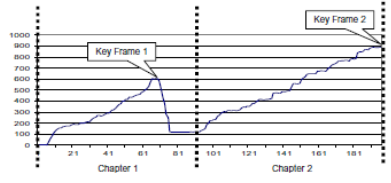
\includegraphics[scale=1]{images/research_mswhiteboard_3}
\caption{Plot of number of stroke cells vs. time.  Key frames are shown at peaks just before stroke count decreases dramatically.}
\end{figure}

\indent \textbf{7.} Color balance is done to make the background uniformly white and increase the color saturation of the pen strokes.  It also reduces image noise.  A final image is presented in Figure 2, below.
\begin{figure}[H]
\centering
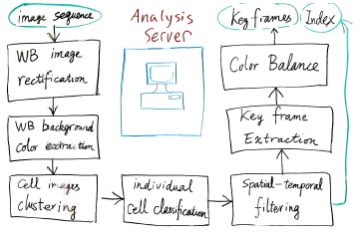
\includegraphics[scale=1]{images/research_mswhiteboard_2}
\caption{Example of a key frame as processed by the WCS}
\end{figure}

\indent Browsing software allows viewing of key frames and audio playback.  Users can zoom in/out and cut and paste the image to other documents.  Double clicking on pen stroke cells plays audio at the time of the time stamp of the cell.  Stroke cells will then be displayed as time progresses in the audio to their respective time stamps. \\
\indent Access to the browsing software is via a token-based access model, where an access URL is emailed to all meeting participants.

	\subsubsection*{Limitations}
For proper functionality, the WCS requires a constant use environment.  The whiteboard must have a constant color, constant lighting, and the camera must have constant exposure settings for the system to work properly.  Most of these factors are standard for a normal whiteboard environment.  However, the research team suggests that if a constant environment could not be guaranteed, the system might still work if a patch of known color were placed in the camera's field of vision, so the system could adjust settings on the fly based on the changes to the constant color patch. \\  \\
	\indent At the time of publication, the team noted that the frame rate of cameras on the market was a limiting factor for the system.  Since this research is 10 years old, this is no longer as limiting - a quick search of competitively priced cameras returned cameras with over twice the frame rate as the PowerShot G2 used here.
Other problems with the system are less likely.  If a person in a white shirt stands perfectly still in front of the board for a long period of time, the system may not deduce that the person is in the foreground.  This is interesting to note, but not a likely occurrence in a lecture environment.    
	
	\subsubsection*{Relevance to ProPANE}
This system, as a whole, is very similar to our final goals for the BU ProPANE system.  Especially useful to us is the key frame idea, since professors using the system will not want to sort through hundreds of images in order to find just a few important ones.  The idea of breaking the board up into cells for analysis is also very interesting to us, as it greatly reduces the processing requirements.  However, it is not perfect for our project.  The WCS is purely a {\sl whiteboard} capture system, whereas our system should work for black boards as well.  Additionally, we are not focusing on any audio capture or playback for our system.

	\subsection*{ReBoard}
Source: {\color{red} \url{http://arxiv.org/ftp/arxiv/papers/0911/0911.0039.pdf}} 
	\subsubsection*{Summary}
ReBoard is a system developed by FX Palo Alto Laboratory, Inc.  It captures whiteboard content both actively and passively, while providing a robust platform for data retrieval and sharing.  Users can browse captured data by aspects such as time or location of capture, or who was present for data capture.  
	\subsubsection*{Key Features}
ReBoard's focus is on the ease of sharing captured data between users.  The User Interface (UI) provides multiple options for data retrieval and sharing.  
\begin{itemize} \itemsep -2pt
	\item \emph{Calendar View:} Sorts images by date of capture, color-coded by type of content (blue for personal, violet for collaborative, etc...).  
	\item \emph{Timeline View:} Arranges captured images chronologically, with a histogram where higher bars mean more content was created or erased for that capture.  Dates at the bottom of the display indicate approximate date of capture.    
	\item \emph{Heatmap View:} Aggregates changes to the board by location over a given time frame.  The more a region of the board has changed, the warmer the color used to fill the region.
	\item \emph{Summary Pane:} Users can click the ``detail'' button for a particular content record to open in a new browser tab.  This view provides a detailed interface for viewing high-resolution images of the captured content and controls to manipulate the associated metadata. 
\end{itemize}
Thanks to these views, users can retrieve data based on who was present during its creation, by a specific region on the whiteboard where it was created, by the time it was created, or by user-assigned labels and descriptions.  \newline
\indent ReBoard's unique feature is its ability to detect collaboration.  The system will detect when multiple people are working at the board, and the content created at that time will be tagged as collaborative, and users can sort images in the UI by this characteristic.  

\begin{figure}[H]
\centering
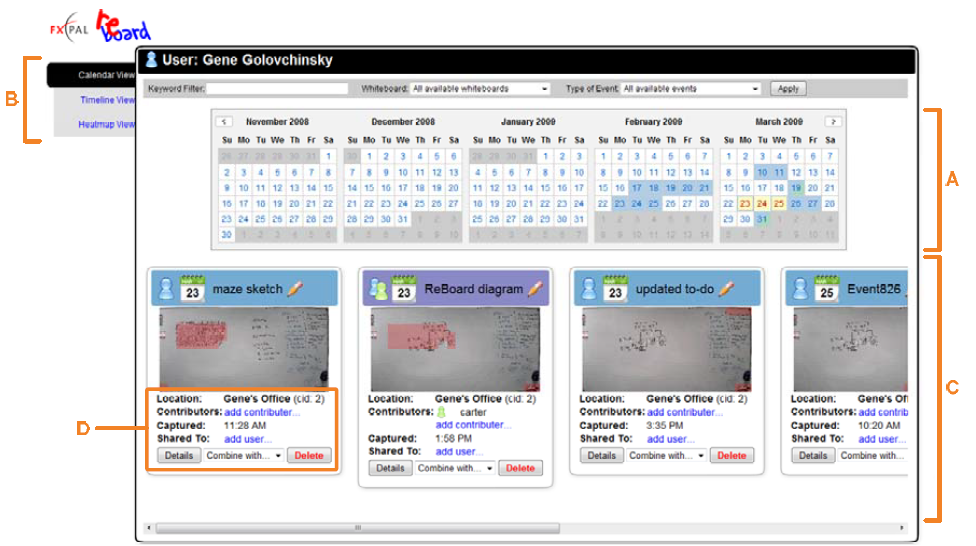
\includegraphics[scale=0.4]{images/research_reboard_1}
\caption{ReBoard's Calendar View}
\end{figure}

\begin{figure}[H]
\centering
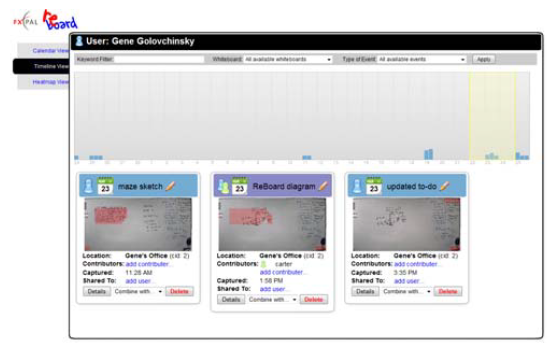
\includegraphics[scale=0.7]{images/research_reboard_2}
\caption{ReBoard's Timeline View}
\end{figure}

\begin{figure}[H]
\centering
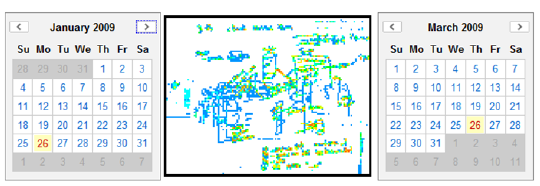
\includegraphics[scale=0.7]{images/research_reboard_3}
\caption{Close-up of ReBoard's Heatmap View}
\end{figure}

	\subsubsection*{Technical information}
The ReBoard system consists of one video camera per whiteboard, an application server, a database to store images and metadata, detectors that sense collaborative activity, detectors that record content changes, and portable user interfaces to manage content and metadata (these are optional).  The video cameras record at 10 fps, with important images captured at times indicated by the detectors and user interfaces.  Cameras are calibrated at installation to correct for geometric distortion due to off-axis camera positioning.  The content change detector is a Java-based service that leverages Java's Media framework and OpenCV's image processing libraries.  The collaboration detector is a C\# Windows Service using the AForge computer vision framework for basic video processing and ``blob'' detection (more information on AForge \href{code.google.com/p/aforge/}{here}).  Event detectors have IDs that link them to a specific camera so they can work independent of each other.  The application server is written in Grails, with the metadata stored in a MySQL database.  The server manages user accounts, sessions and access control, and exposes a set of REST-like web services for AJAX UI clients and for communicating with the event detectors. The persistent UI runs on a portable Chumby device (more information \href{http://en.wikipedia.org/wiki/Chumby}{here}).  It allows for manual image capture, capure disable, and content bookmark.  The persistent UI is not necessary for the system to function.

\begin{figure}[H]
\centering
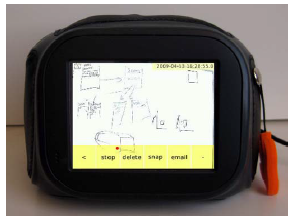
\includegraphics[scale=1]{images/research_reboard_4}
\caption{Persistent UI running on a Chumby device}
\end{figure}

	\subsubsection*{Relevance to ProPANE}
While ReBoard is designed for continuous use in the workplace, as opposed to ProPANE's classroom setting, there are still some features of the ReBoard system that could contribute to the ProPANE system.  The portable user interface is an interesting concept, because while the ProPANE system should be fully automatic, the ability to manually capture board images would be useful as a kind of fail-safe if problems arose with automatic detection.  Another strength of ReBoard is its web UI.  The option of multiple views to recover data seems very useful, and some would be particularly useful to ProPANE.  The calendar view would make it easy to sort lectures by date, and a modified timeline view with exact dates would help professors identify lectures with more content than others.  Finally, the heatmap view could be utilized on a smaller scale to track changes during one particular lecture.   


  \subsection*{Cameras we could use in our project}
Here are the current top three cameras that we think could help us the most when building our image capturing system.

\begin{itemize}
    \item Nikon COOLPIX S800c 16 MP Digital Camera
    \begin{itemize}
        \item \url{http://www.amazon.com/Nikon-COOLPIX-Digital-Optical-3-5-inch/dp/B0090SLKUM}
    \end{itemize}
    \item Samsung Camera EK-GC100 Galaxy Camera
    \begin{itemize}
        \item \url{http://pdadb.net/index.php?m=specs&id=3813&c=samsung_ek-gc100_galaxy_camera}
    \end{itemize}
    \item Polaroid SC1630 Smart Camera
    \begin{itemize}
        \item \url{http://www.upi.com/Science_News/2012/01/16/Polaroid-joins-digital-camera-arena/UPI-61851326750025/}
    \end{itemize}
\end{itemize}

We are interested in them because they are cameras running the Android operating system. This means that we could create our own custom application for these devices, greatly simplifying our design process. These cameras would also be useful because they can connect to Bucknell's wifi network. This would allow us to wirelessly transferr information from the cameras to whatever image processing hardware we decide to connect it to. The main drawbacks at the moment with these Android cameras is that two of them haven't been released yet (Samsung and Polaroid). IF they are released in time, they would be the most desireable of the various camera options available.

\subsection*{Details on Learning Disabilaties}
        \subsubsection*{Introduction}
One of the major motivating factors behind designing our image capturing system is to help meet the needs of students with disabilities. The term "students with disabilities" is a very broad term, however, so we would like to use the following section to help discribe some of the things that mildly disabled students have trouble with at Bucknell, and would therefore need our system to capture information presented on the board for them.
\\
Source: \\
{\color{red} \url{http://www.sfasu.edu/disabilityservices/facultyandstaff/for_service_providers/note_q_a.asp}} \\
\\
Disabilities that students might have that impair their ability to take notes:
    \begin{itemize}
        \item Visual Impairments
        \begin{itemize}
            \item May be fully blind and need notes translated into Braille
            \item May not see well and need large print letters
            \item May have trouble copying information from whiteboards, projectors, etc.
            \item May have trouble seeing certain colors when framed by a white or black background
        \end{itemize}
        \item Specific Learning Disabilities
        \begin{itemize}
            \item Reading Disability
            \item Writing Disability
            \item Spelling Disability
            \item Inability to copy what they see
            \item Inability to write what they hear
            \item Inability to write legibly
            \item Number Reversal problems
        \end{itemize}
        \item Mobility Impairments
        \begin{itemize}
            \item Physically unable to write
            \item Physically unable to write quickly
            \item May be unable to effectively handle a writing impliment
        \end{itemize}
        \item Partial or Full loss of hearing
    \end{itemize}

This is just a small portion of the many disabilities faced by students in universities around the world. We hope to help them by giving them full access all information presented on boards during lectures. By providing easily accessible, easily modifiable images, we hope to help even the playing field for students with disabilites.
Secondary goals of our project will help to make the learning process even easier. Some students get distracted if they see more than one line of text at a time. If we have enough time we will help these students by providing slide bars that will cover portions of the images that students are not currently viewing. This and many other minor features are things that we will accomplish if we have free time after completing our primary objectives.


\end{document}
